\documentclass[11pt]{article}

\newcommand{\yourname}{}
\newcommand{\yourcollaborators}{}

\def\comments{0}

%format and packages%\usepackage{algorithm, algorithmic}
\usepackage{algpseudocode}
\usepackage{amsmath, amssymb, amsthm}
\usepackage{enumerate}
\usepackage{enumitem}
\usepackage{framed}
\usepackage{verbatim}
\usepackage[margin=1.0in]{geometry}
\usepackage{multirow}

\usepackage{microtype}


\usepackage{graphicx}
\usepackage{tikz}
\usetikzlibrary{automata, positioning, arrows.meta}

	\definecolor{processblue}{cmyk}{0.96,0,0,0}


\usepackage{kpfonts}
\usepackage{palatino}
	\DeclareMathAlphabet{\mathtt}{OT1}{cmtt}{m}{n}
	\SetMathAlphabet{\mathtt}{bold}{OT1}{cmtt}{bx}{n}
	\DeclareMathAlphabet{\mathsf}{OT1}{cmss}{m}{n}
	\SetMathAlphabet{\mathsf}{bold}{OT1}{cmss}{bx}{n}
	\renewcommand*\ttdefault{cmtt}
	\renewcommand*\sfdefault{cmss}
	\renewcommand{\baselinestretch}{1.06}
\usepackage{tikz}
	\usetikzlibrary{positioning}
	\definecolor{processblue}{cmyk}{0.96,0,0,0}
    \usetikzlibrary{matrix,arrows}

\tikzset{
->, % makes the edges directed
>=Stealth, % makes the arrow heads bold
node distance=3cm, % specifies the minimum distance between two nodes. Change if necessary.
every state/.style={thick, fill=gray!10}, % sets the properties for each ’state’ node
initial text=$ $, % sets the text that appears on the start arrow
}
	
\usepackage{hyperref}

\hypersetup{
	linktocpage=true,
	colorlinks=true,				% false: boxed links; true: colored links
	linkcolor=blue,		% color of internal links
	citecolor=blue,	% color of links to bibliography
	urlcolor=blue,		% color of external links
}

\usepackage[boxruled,vlined,nofillcomment]{algorithm2e}
	\SetKwProg{Fn}{Function}{\string:}{}
	\SetKwFor{While}{While}{}{}
	\SetKwFor{For}{For}{}{}
	\SetKwIF{If}{ElseIf}{Else}{If}{:}{ElseIf}{Else}{:}
	\SetKw{Return}{Return}

%enclosure macros
\newcommand{\paren}[1]{\ensuremath{\left( {#1} \right)}}
\newcommand{\bracket}[1]{\ensuremath{\left\{ {#1} \right\}}}
\renewcommand{\sb}[1]{\ensuremath{\left[ {#1} \right\]}}
\newcommand{\ab}[1]{\ensuremath{\left\langle {#1} \right\rangle}}

%probability macros
\newcommand{\ex}[2]{{\ifx&#1& \mathbb{E} \else \underset{#1}{\mathbb{E}} \fi \left[#2\right]}}
\newcommand{\pr}[2]{{\ifx&#1& \mathbb{P} \else \underset{#1}{\mathbb{P}} \fi \left[#2\right]}}
\newcommand{\var}[2]{{\ifx&#1& \mathrm{Var} \else \underset{#1}{\mathrm{Var}} \fi \left[#2\right]}}

%useful CS macros
\newcommand{\poly}{\mathrm{poly}}
\newcommand{\polylog}{\mathrm{polylog}}
\newcommand{\zo}{\{0,1\}}
\newcommand{\pmo}{\{\pm1\}}
\newcommand{\getsr}{\gets_{\mbox{\tiny R}}}
\newcommand{\card}[1]{\left| #1 \right|}
\newcommand{\set}[1]{\left\{#1\right\}}
\newcommand{\negl}{\mathrm{negl}}
\newcommand{\eps}{\varepsilon}
\DeclareMathOperator*{\argmin}{arg\,min}
\DeclareMathOperator*{\argmax}{arg\,max}
\newcommand{\eqand}{\qquad \textrm{and} \qquad}
\newcommand{\ind}[1]{\mathbb{I}\{#1\}}
\newcommand{\sslash}{\ensuremath{\mathbin{/\mkern-3mu/}}}

%mathbb
\newcommand{\N}{\mathbb{N}}
\newcommand{\R}{\mathbb{R}}
\newcommand{\Z}{\mathbb{Z}}
%mathcal
\newcommand{\cA}{\mathcal{A}}
\newcommand{\cB}{\mathcal{B}}
\newcommand{\cC}{\mathcal{C}}
\newcommand{\cD}{\mathcal{D}}
\newcommand{\cE}{\mathcal{E}}
\newcommand{\cF}{\mathcal{F}}
\newcommand{\cL}{\mathcal{L}}
\newcommand{\cM}{\mathcal{M}}
\newcommand{\cO}{\mathcal{O}}
\newcommand{\cP}{\mathcal{P}}
\newcommand{\cQ}{\mathcal{Q}}
\newcommand{\cR}{\mathcal{R}}
\newcommand{\cS}{\mathcal{S}}
\newcommand{\cU}{\mathcal{U}}
\newcommand{\cV}{\mathcal{V}}
\newcommand{\cW}{\mathcal{W}}
\newcommand{\cX}{\mathcal{X}}
\newcommand{\cY}{\mathcal{Y}}
\newcommand{\cZ}{\mathcal{Z}}

\newcommand{\opt}{\textsc{opt}}

%theorem macros
\newtheorem{thm}{Theorem}
\newtheorem{lem}[thm]{Lemma}
\newtheorem{fact}[thm]{Fact}
\newtheorem{clm}[thm]{Claim}
\newtheorem{rem}[thm]{Remark}
\newtheorem{coro}[thm]{Corollary}
\newtheorem{prop}[thm]{Proposition}
\newtheorem{conj}[thm]{Conjecture}

\theoremstyle{definition}
\newtheorem{defn}[thm]{Definition}


\newcommand{\instructor}{Drew van der Poel}
\newcommand{\hwnum}{3}
\newcommand{\hwdue}{Friday, July 29 at 11:59pm via \href{https://www.gradescope.com/courses/406943}{Gradescope}}

\theoremstyle{theorem}
\newtheorem{prob}{Problem}
\newtheorem{sol}{Solution}

\definecolor{cit}{rgb}{0.05,0.2,0.45} 
\newcommand{\solution}{\medskip\noindent{\color{blue}\textbf{Solution:}}}

\begin{document}
{\Large 
\begin{center}{CS3800: Theory of Computation} --- Summer II '22 --- \instructor \end{center}}
{\large
\vspace{10pt}
\noindent Homework~\hwnum \vspace{2pt}\\
Due~\hwdue}

\bigskip
{\large
\noindent Name: \yourname \vspace{2pt}\\ Collaborators: \yourcollaborators}

\vspace{15pt}
\begin{itemize}

\item Make sure to put your name on the first page.  If you are using the \LaTeX~template we provided, then you can make sure it appears by filling in the \texttt{yourname} command.

\item This assignment is due~\hwdue.  No late assignments will be accepted.  Make sure to submit something before the deadline.

\item Solutions must be typeset.  If you need to draw any diagrams, you may draw them by hand as long as they are embedded in the PDF.  I recommend using the source file for this assignment to get started.

\item I encourage you to work with your classmates on the homework problems. \emph{If you do collaborate, you must write all solutions by yourself, in your own words.}  Do not submit anything you cannot explain.  Please list all your collaborators in your solution for each problem by filling in the \texttt{yourcollaborators} command.

\item Finding solutions to homework problems on the web, or by asking students not enrolled in the class is strictly forbidden.

\end{itemize}


\newpage

\begin{prob} Context-Free Grammars (\emph{7 points})\end{prob}

In the following problems, the alphabet $\Sigma = \{a, b\}$. Give a context-free grammar for each of the following languages.

\begin{enumerate}[label=(\alph*)]

\item \textbf{[3 pts.]}  $L_a = \{a^nb^n | n > 1$ is not a multiple of 3$\}$

Show how to generate $aaaabbbb$ with your grammar.

\solution

A $\rightarrow$ aabb $|$ aaaAbbb $|$ aaAbb  \\~\\

To generate $aaaabbbb$: A $\rightarrow$ aaAbb $\rightarrow$ aaaabbbb

\item \textbf{[4 pts.]}  $L_a = \{w | w \text{~has twice as many a's as b's}\}$

Show how to generate $aababaaab$ and $aaaabb$ with your grammar.

\solution

A $\rightarrow$ AA $|$ aAbAa $|$ aaAbA $|$ AbAaa $|$ $\varepsilon$ \\~\\

To generate $aababaaab$: A $\rightarrow$ AA $\rightarrow$ (aaAbA)(A) $\rightarrow$ (aaAbA)(AA) $\rightarrow$ (aaAbA)(aAbAa)(A) $\rightarrow$ (aaAbA)(aAbAa)(AA) $\rightarrow$ (aaAbA)(aAbAa)(aaAbA)(A) $\rightarrow$ (going to skip a few steps and replace all of the A's with the empty string) $\rightarrow$
aababaaab

To generate $aaaabb$: A $\rightarrow$ aaAbA $\rightarrow$ aa(aaAbA)bA $\rightarrow$ (skipping a few steps, replacing all of the A's with the empty string)
$\rightarrow$ aaaabb







\newpage

\begin{prob} CFGs and PDAs (\emph{7 points})\end{prob}

Consider the following context-free grammar $G$:

$S \rightarrow aWb | bWa$

$W \rightarrow aW | bW | \epsilon$

\begin{enumerate}[label=(\alph*)]

\item \textbf{[2 pts.]} Describe the set of strings which can be generated by $G$.

olution 

The set of all strings in which the first input is $a$ and the last input is $b$ or the first input is $b$ and the last input is $a$.

\item \textbf{[5 pts.]} Give a PDA which recognizes the language given by grammar $G$. You should show all necessary states for ``guessing" rule $S$, but can use shorthand otherwise. Specify $\Sigma$ and $\Gamma$.

\solution

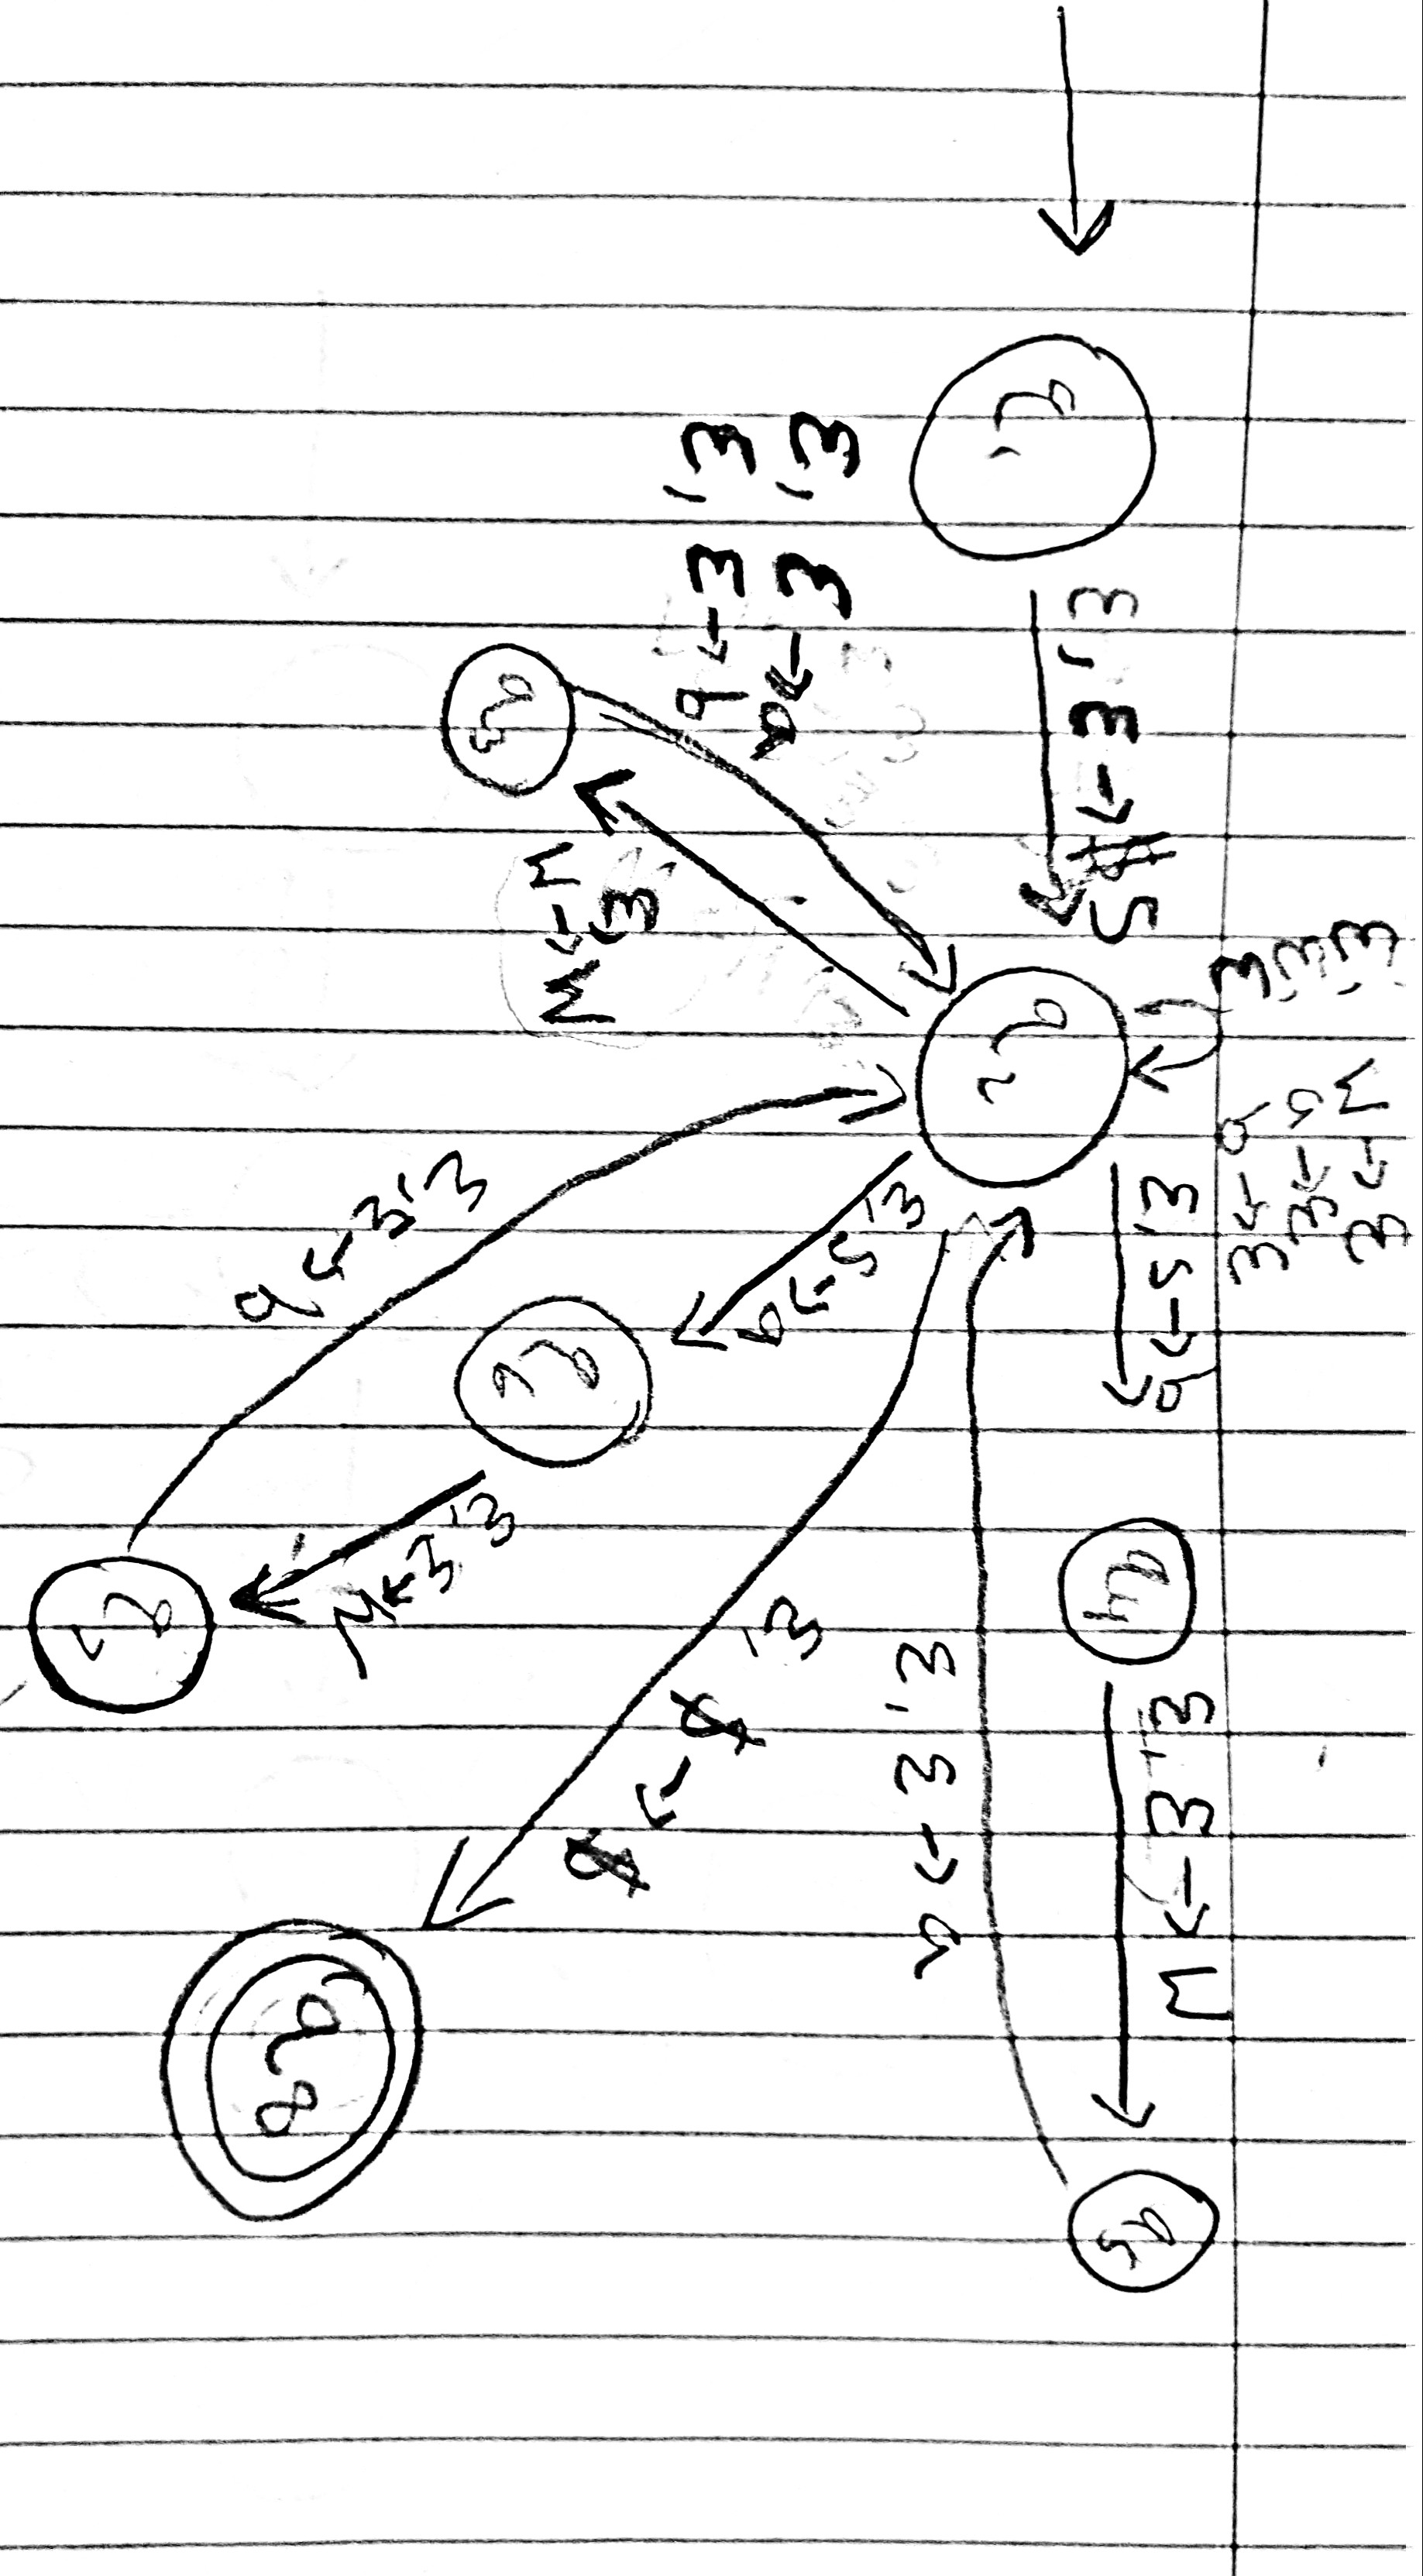
\includegraphics[angle=270,origin=c, scale=0.12]{./p2/hw3q2b.jpg}

$\Sigma$ = $\{a, b\}$ \\
$\Gamma$ = $\{S, W, a, b\}$ 






\end{enumerate}


\newpage

\begin{prob} PDAs (\emph{8 points})\end{prob}

Consider $\Sigma = \{0,1\}$ and language $L = \{0^n101^m | n > m; n, m \in \mathbb{N}\}$.

Show that $L$ is context-free by giving a PDA which recognizes it.
You should give a complete PDA. Your machine should accept strings $00000001011$, $010$, $00101$, and $00000010$, but not $10$ $0010111$, or $0101$ . Explain why it accepts $00101$ and why it does not accept $0101$.

\solution 

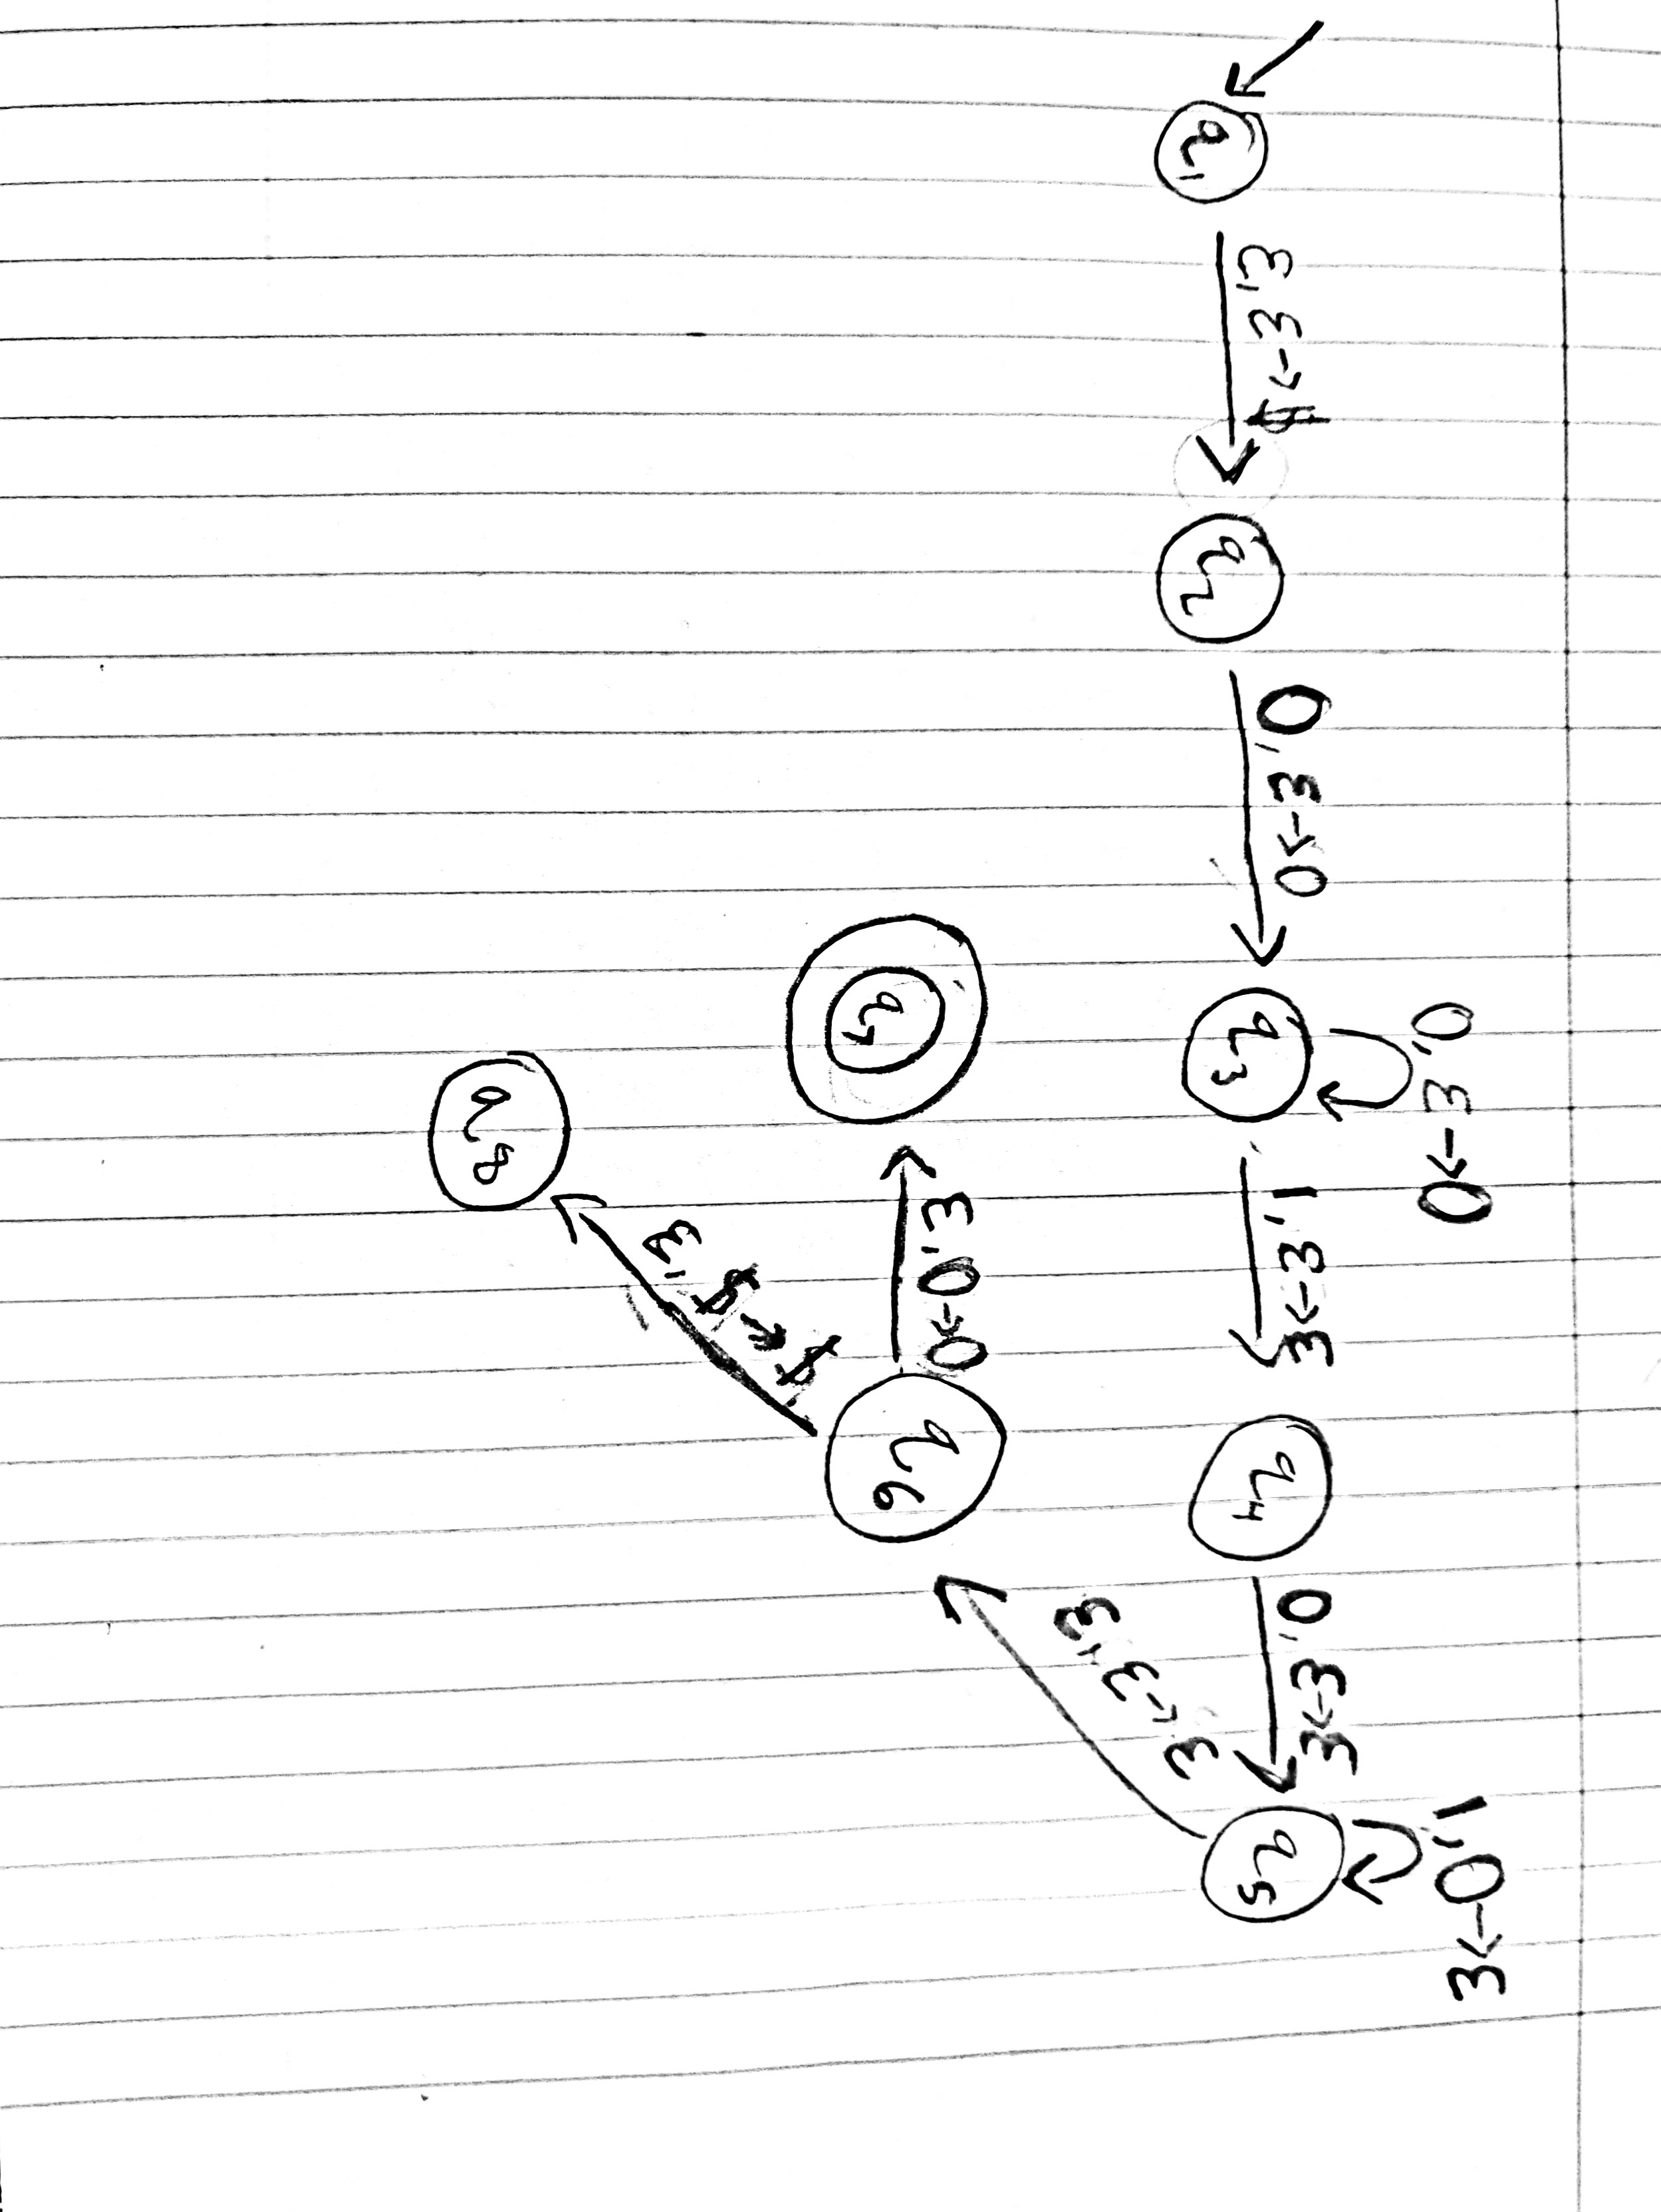
\includegraphics[angle=90,origin=c, scale=0.15]{./p3/hwp3.jpg}


$00101$: We start at $q1$, and epsilon transition while initializing the stack to $q2$. At $q2$, we read the first 0 and push it onto the stack to transition to $q3$. At $q3$, we read the next 0 and push it onto the stack, staying at $q3$. Again, at $q3$, the next input is 1, so we take the 1 transition to $q4$ while pushing nothing onto the stack. At $q4$, our next input is 0 so we transition to $q5$ and push nothing to the stack.
At $q5$ we break into two branches, one where read the last input, 1, stay at $q5$ and remove a 0 off of the stack or we can take the epsilon transition to $q7$: 
If we take the epsilon transition, then we would end up at $q6$ and then since the top of our stack is a 0, we can take the epsilon transition to $q7$. Since in this case we still have a 1 to read and there are no transitions in $q7$ for the 1 then this branch fails.
If we take the $q5$ transition and remove a 0 off of the stack, then we can take the transition $q6$ and then since the top of our stack is still a 0, we can take the epsilon transition to $q7$. At $q7$, since we are finished with reading the string and we are in an accept state, the string is accepted. \\~\\

$0101$: We start at $q1$, and epsilon transition while initializing the stack to $q2$. At $q2$, we read the first 0 and push it onto the stack to transition to $q3$. At $q3$ we read the 1 to transition to $q4$ and then the 0 to transition to $q5$, pushing nothing onto the stack in both transitions.
At $q5$, we once again break into two branches: one where we take the epsilon branch and one where we stay at $q5$, read the 1, and pop a 0 off of the stack. For the same reason, taking the epsilon transition would result in the branch rejecting at $q7$. In the other branch, after we read the 1 and popped the top 0 off of the stack, then we can take the epsilon transition to $q6$. At $q6$, since our stack is now empty, we take the transition to $q8$ where the string will be rejected.









\newpage

\begin{prob} Non Context-Free Languages (\emph{4+4=8 points})\end{prob}

\begin{enumerate}[label=(\alph*)]

\item Prove that language $L = \{w | w \in \{a,b,c\}^*$ and the number of a's is equal to the number of b's and the number of a's is greater than the number of c's$\}$ is not context-free.

\solution \\
Assume that $L$ is a context-free grammar, and so the context-free grammar pumping lemma applies. Let $P$ be the pumping length. Let $S = a^{2P}c^{P}b^{2P}$,  $S$ $\subseteq$ $L$, and $|S| \geq P$. Because we know that $|vxy| \leq P$, $vxy$ cannot have both a's and b's. We can then break the string of $vy$ into 2 cases: \\

Case 1: $vy$ contains all of the same letters. If $vy$ consists of all a's or all b's then if we let $i = 2$, $uvvxyyz$, then the string is no longer in the language since either $|a| > |b|$ or $|b| > |a|$ depending on the scenario. If $vy$ consists of only c's then if we let $i = P$, $uv^Pxy^Pz$, then we know that $|c| > |a|$ which means that $S$ is no longer in the language. \\ 

Case 2: $vy$ contains some mix of a's and c's or b's and c's. If this is the case then if we let $i = 2$, $uvvxyyz$, we will have an unequal number of a's and c's depending on the scenario. If $vy$ is some mixture of a's and c's then we will have more a's than c's after pumping and if $vy$ consists of only b's and c's then we will have more c's than a's after pumping. \\

Thus, by contradiction, the string $S$ cannot uphold the pumping lemma despite being in the grammar, $L$, which means that $L$ is not context-free.
\item Prove that language $L = \{a^l b^{l^2} | l \in \mathbb{N}\}$ is not context-free.

\solution \\
Assume that $L$ is a context-free grammar, and so the context-free pumping lemme applies. Let $P$ be the pumping length. Let $S = a^Pb^{P^2}$, $S$ $\subseteq$ $L$, and $|S| \geq P$. Because we know that $|vxy| \leq P$, $vxy$ either can be all a's, all b's or, a mixture of a's and b's. \\

Case 1: $vxy$ consists of all a's. We know that $vy$ is non-empty ($|vy| > 0$), so if we let $i = 2$, $uvvxyyz$, must mean that the number of a's must increase. Since the number of a's increased by some arbitrary amount and the number of b's has not changed, then $|a|$ is no longer equal to $\sqrt{|b|}$ which means $uvvxyyz$ is not in $L$. This means that $S$ does not uphold the pumping lemma for this case. \\

Case 2: $vxy$ consists of all b's. We know that $vy$ is non-empty ($|vy| > 0$), so if we let $i = 2$, $uvvxyyz$, must mean that the number of b's must increase. Since the number of b's increased by some arbitrary amount and the number of a's has not changed, then $|b|$ has to now be greater than the $|a|^2$ which means $uvvxyyz$ is not in $L$. This means that $S$ does not uphold the pumping lemma for this case. \\

Case 3: $vxy$ consists of some mix of a's and b's. If we let, $i = 2$, we know that the number of a's and b's must increase by some arbitrary amount.  If we let $j$ be the number of 0's in $vxy$ then the number of 1's in $vxy$ is $P - j$
\end{enumerate}



\end{enumerate}






\end{document}
